\sectionbreak \section*{
  \gostTitleFont
  \redline
  1. ОБЩАЯ ХАРАКТЕРИСТИКА ПРЕДПРИЯТИЯ
}

\titlespace

\subsection*{ 
  \gostTitleFont
  \redline
  1.1 Изучение структуры предприятия
} 

\subtitlespace

{\gostFont

  \par \redline Организационная структура - это схема, отражающая иерархию управления и взаимосвязи между различными подразделениями и должностями внутри организации. Она показывает, как устроено управление компанией, кто кому подчиняется, какие подразделения существуют и как они взаимодействуют. Это "скелет" организации, определяющий ее формальные коммуникации и потоки информации.

  \par \redline \textbf{Организационная структура ОАО «Савушкин продукт»}

  \par \redline ОАО «Савушкин продукт» представляет собой крупное производственное объединение, включающее 6 высокотехнологичных производственных площадок, расположенных в Бресте, Пинске, Столине, Берёзе, Ивацевичах и Барановичах. Организационная структура предприятия построена по территориально-производственному принципу.

  \par \redline Во главе предприятия стоит генеральный директор, которому подчиняются несколько заместителей по различным направлениям деятельности. Каждое функциональное направление представлено отдельным подразделением, а именно:
  
  \par \redline • Производственный департамент;
  \par \redline • Финансовое управление;
  \par \redline • Отдел сбыта и маркетинга;
  \par \redline • Отдел информационных технологий;
  \par \redline • Юридический отдел;
  \par \redline • Отдел кадров.

  \par \redline Внутри этих крупных подразделений выделены дополнительные структурные единицы, такие как секторы, группы, бюро. Управление предприятием осуществляется через головной офис, расположенный в Бресте. В структуру управления также входят:
  
  \par \redline • Совет директоров;
  \par \redline • Генеральная дирекция;
  \par \redline • Производственная дирекция;
  \par \redline • Коммерческая дирекция;
  \par \redline • Финансовая дирекция;
  \par \redline • Служба качества;
  \par \redline • Техническая дирекция.

  \par \redline Товаропроводящая сеть компании включает 6 торговых филиалов в Беларуси (Минск, Гомель, Витебск, Могилёв, Гродно, Брест) и торговый дом в Москве. Каждый филиал имеет собственную структуру управления, подчиняющуюся головному офису.

  \par \redline Производственные площадки имеют следующие основные подразделения:
  
  \par \redline • Производственные цеха;
  \par \redline • Лаборатории контроля качества;
  \par \redline • Складские комплексы;
  \par \redline • Инженерно-технические службы;
  \par \redline • Административно-хозяйственные отделы.

  \par \redline Все производственные площадки сертифицированы по международным стандартам СТБ ISO 9001-2015, ISO 14001, ISO 45001 и FSSC 22000, что определяет высокий уровень организации производственных и управленческих процессов.

  \par \redline \textbf{Функциональная структура ОАО «Савушкин продукт»}

  \par \redline Функциональная структура - это способ организации деятельности предприятия, при котором каждое подразделение специализируется на выполнении определенных функций или задач. Она ориентирована на специализацию и разделение труда, что позволяет повысить профессионализм сотрудников и эффективность выполнения отдельных операций и процессов.

  \par \redline Основные преимущества функциональной структуры ОАО "Савушкин продукт":
  \par \redline • Высокая компетентность сотрудников в своей области;
  \par \redline • Четкое распределение ответственности;
  \par \redline • Возможность контроля качества работ;
  \par \redline • Оперативность решения узких, специализированных задач.

  \par \redline Функциональная структура на ОАО "Савушкин продукт" имеет следующее распределение задач и ответственности:
  \par \redline • Производственный департамент отвечает за организацию и управление производственными процессами на предприятии;
  \par \redline • Финансовое управление занимается финансовым планированием, учетом и контролем;
  \par \redline • Отдел сбыта и маркетинга отвечает за продвижение продукции и взаимодействие с клиентами;
  \par \redline • Отдел информационных технологий разрабатывает и внедряет информационные системы, а также обеспечивает техническую поддержку;
  \par \redline • Юридический отдел осуществляет правовое сопровождение деятельности предприятия;
  \par \redline • Отдел кадров занимается управлением персоналом.

  \par \redline В составе технической дирекции функционирует Бюро перспективных разработок, выполняющее стратегическую функцию по поиску, разработке и внедрению инноваций. К основным задачам Бюро относится разработка и поддержка инновационных инструментов управления предприятием, создание систем описания технологических процессов, изучение новых технологий для повышения эффективности производства.

  \par \redline \textbf{Взаимосвязь организационной и функциональной структур}

  \par \redline Таким образом, организационная структура определяет иерархию управления, а функциональная - распределение задач и ответственности между различными подразделениями ОАО «Савушкин продукт». Предприятие построено по принципу вертикальной интеграции с четким распределением функций между подразделениями и эффективной системой управления, что обеспечивает успешное функционирование предприятия как единого производственного комплекса.

  \par
}

\subtitlespace

\subsection*{ 
  \gostTitleFont
  \redline
  1.2 Изучение должностных инструкций работников подразделения
} 

\subtitlespace

{\gostFont

  \par \redline В процессе прохождения практики в компании ООО "Савушкин продукт" одной из важных задач являлось изучение должностных инструкций работников подразделения. Ознакомление с данными документами позволяет понять функциональные обязанности, права, ответственность и квалификационные требования к сотрудникам, что способствует более эффективному вхождению в рабочий процесс. Должностные инструкции играют важную роль в организации труда и обеспечении выполнения поставленных задач. 

  \par \redline Подразделение, в котором проходила практика, — бюро перспективных разработок, занимается автоматизированными системами управления технологическими процессами (АСУТП). Основными задачами отдела являются:

  \par \redline • Разработка, внедрение и сопровождение АСУТП на предприятии;
  \par \redline • Обслуживание программного обеспечения для автоматизации технологических процессов;
  \par \redline • Диагностика и устранение неисправностей в программном обеспечении;
  \par \redline • Обеспечение информационной безопасности систем управления;
  \par \redline • Техническая поддержка пользователей АСУТП.
  \par \redline В подразделении работают следующие категории сотрудников:
  \par \redline • Руководитель отдела программирования;
  \par \redline • Программисты АСУТП;
  \par \redline • Инженеры по автоматизации;
  \par \redline • Системные администраторы АСУТП.
  \par \redline В ходе изучения были рассмотрены должностные инструкции следующих работников:
  \par \redline • Руководителя отдела программирования;
  \par \redline • Программиста АСУТП;
  \par \redline • Инженера по автоматизации.
  \par \redline Руководитель отдела программирования отвечает за организацию работы отдела, распределение задач между сотрудниками, контроль выполнения поставленных задач, обеспечение соблюдения политики информационной безопасности и взаимодействие с другими подразделениями предприятия.
  \par \redline Программист АСУТП занимается разработкой программного обеспечения для автоматизации технологических процессов, написанием программ для контроллеров, тестированием программного обеспечения и его внедрением в производственные процессы. Основные обязанности программиста АСУТП включают:
  \par \redline • Разработка алгоритмов управления технологическими процессами;
  \par \redline • Программирование контроллеров;
  \par \redline • Тестирование программного обеспечения;
  \par \redline • Ведение технической документации;
  \par \redline • Поддержка и обслуживание программного обеспечения АСУТП.
  \par \redline Инженер по автоматизации отвечает за настройку и наладку оборудования АСУТП, интеграцию программного обеспечения с аппаратной частью и проведение диагностики систем. Его обязанности включают:
  \par \redline • Настройку контроллеров и интерфейсов;
  \par \redline • Монтаж и обслуживание датчиков и исполнительных механизмов;
  \par \redline • Тестирование систем автоматизации;
  \par \redline • Взаимодействие с программистами для устранения ошибок;
  \par \redline • Подготовку технической документации.

  \par \redline Должностные инструкции являются основой для распределения обязанностей между сотрудниками, что позволяет четко определить сферу ответственности каждого работника. Они способствуют соблюдению трудовой дисциплины, помогают избежать дублирования функций и обеспечивают контроль качества выполняемой работы.

  \par \redline На практике инструкции помогают оперативно решать возникающие задачи, так как каждый сотрудник знает свои обязанности и зону ответственности. 

  \par 
}


\subtitlespace

\subsection*{  
  \gostTitleFont
  \redline
  1.3 Обзор задач, решаемых подразделением
} 

\subtitlespace

{\gostFont

  \par \redline На ОАО «Савушкин продукт», можно отметить следующее распределение задач и ответственности:
  \par \redline - Производство продукции: выпуск молочных товаров (йогурты, сыры, творог, молоко);
  \par \redline - Контроль качества и безопасность: соблюдение строгих стандартов;
  \par \redline - Логистика и снабжение: управление цепочками поставок сырья и готовой продукции;
  \par \redline - Инновации: внедрение новых технологий и разработка продуктов;
  \par \redline - Экология и устойчивое развитие: минимизация экологического следа;
  \par \redline - Социальная ответственность: поддержка местных сообществ и сотрудников.

  \par \redline Производственные задачи:
  \par \redline - Оптимизация производственных процессов. Подразделение решает задачи повышения эффективности линий, снижения энергозатрат и увеличения объемов выпуска. Например, автоматизация упаковки позволила сократить время обработки заказов на 15\%;
  \par \redline - Расширение ассортимента. Разработка новых продуктов, таких как линейки органических йогуртов или безлактозных сыров, отвечает запросам рынка. В 2023 году брестский филиал запустил производство сыра с пробиотиками, что стало ответом на тренд здорового питания;
  \par \redline - Соблюдение стандартов. Производство соответствует требованиям ISO, ХАССП и белорусским ГОСТам, что критически важно для экспорта в ЕАЭС и другие страны.

  \par \redline Контроль качества и безопасность:
  \par \redline - Многоуровневый контроль. Каждая партия проходит лабораторные испытания на микробиологические и физико-химические показатели. Внедрена система отслеживания сырья от поставщика до прилавка;
  \par \redline - Работа с рекламациями. Подразделение оперативно реагирует на обратная связь от потребителей, анализируя причины дефектов и корректируя процессы;
  \par \redline - Сертификация. Поддержка международных сертификатов (например, Halal, Orga- nic) расширяет возможности экспорта.

  \par \redline Логистика и снабжение:
  \par \redline - Управление поставками сырья. Сотрудничество с местными фермерскими хозяйствами обеспечивает стабильность поставок молока-сырья. Внедрена цифровая платформа для прогнозирования спроса;
  \par \redline - Дистрибуция готовой продукции. Оптимизация маршрутов доставки снизила логистические издержки на 10\%. Подразделение взаимодействует с сетями супермаркетов в Беларуси, России, Казахстане;
  \par \redline - Складское хозяйство. Использование систем WMS (Warehouse Management System) повысило точность учета и скорость отгрузки.

  \par \redline Инновации и развитие:
  \par \redline - Внедрение технологий. На заводе в Бресте используются роботизированные линии розлива, IoT-датчики для мониторинга оборудования;
  \par \redline - Исследования и разработки. Локальный R\&D-центр тестирует новые рецептуры, например, растительно-молочные гибриды для веганского рынка;
  \par \redline - Цифровизация. Внедрение ERP-системы интегрировало производство, логистику и финансы, сократив время согласований.

  \par \redline Экологическая ответственность:
  \par \redline - Снижение отходов. Переход на биоразлагаемую упаковку и переработка 95\% производственных отходов;
  \par \redline - Энергоэффективность. Установка солнечных панелей и рекуперация тепла от оборудования сократили углеродный след на 20\%;
  \par \redline - Водопользование. Система замкнутого цикла очистки воды уменьшила ее потребление на 30\%.

  \par \redline Социальные инициативы:
  \par \redline - Поддержка сотрудников. Программы обучения, медицинское страхование, корпоративный детский сад;
  \par \redline - Участие в жизни региона. Спонсорство школ, экологические акции (посадка деревьев), продовольственная помощь нуждающимся;
  \par \redline - Развитие местной экономики. Закупки сырья у брестских фермеров создают рабочие места в регионе.

  \par \redline Брестское подразделение ОАО «Савушкин продукт» решает комплекс задач, направленных на укрепление позиций компании как локального и международного игрока. Через инновации, качество и ответственность подразделение вносит вклад в устойчивое развитие бизнеса и общества. Дальнейшие цели включают углубление цифровизации, расширение экспорта и усиление экологических инициатив, что соответствует глобальным трендам и стратегии компании.

  \par
}

\subtitlespace

\subsection*{
  \gostTitleFont
  \redline
  1.4 Обзор используемых технических средств на предприятии
} 

\subtitlespace

{\gostFont

  \par \redline На предприятии "Савушкин" в рамках автоматизации производственных процессов используется комплексная система автоматизации, состоящая из программного комплекса SCADA, программно-технического управляющего комплекса PTUSA и инструмента проектирования EasyEPLANner. Бюро перспективных разработок активно участвует в развитии и совершенствовании этих систем.

  \par \redline Рассмотрим аппаратное обеспечение, используемое на предприятии. Основу системы управления составляют программируемые логические контроллеры Phoenix Contact PLCnext серии AXC F 2152 и контроллеры WAGO PFC200, обеспечивающие гибкую платформу для реализации систем управления. Также используются промышленные компьютеры с операционными системами Linux для выполнения программы управления ptusa\_main и различные модули ввода-вывода для подключения датчиков и исполнительных механизмов.

  \par \redline Для контроля технологических процессов применяются различные датчики: температуры, давления, расходомеры для измерения объемов перекачиваемых продуктов, уровнемеры для контроля наполнения емкостей. Управление потоками осуществляется с помощью клапанов и задвижек с электроприводами, а для управления электродвигателями насосов и мешалок используются частотные преобразователи.

  \par \redline Сетевая инфраструктура предприятия включает промышленные коммутаторы для организации сети Ethernet, преобразователи интерфейсов для подключения устройств с различными протоколами связи и оптоволоконные линии связи для обеспечения надежной передачи данных между удаленными участками. Серверное оборудование представлено серверами для размещения SCADA-системы и баз данных, рабочими станциями операторов для мониторинга и управления технологическими процессами, а также системами резервного копирования для обеспечения сохранности данных.

  \par \redline Программное обеспечение предприятия включает несколько ключевых компонентов. Программный комплекс SCADA состоит из серверной части EasyServer для обработки и хранения данных, клиентской части Monitor для визуализации и управления технологическими процессами, редактора конфигурации базы данных DBXmlEditor и ряда вспомогательных библиотек: buglog.dll для ведения журнала ошибок, ConnectionLog.dll для регистрации подключений, MSUniServ.dll для универсального сервиса, ClientPLog.dll и ClientTLog.dll для ведения журналов, PGPropServ.dll и propservice.dll для работы с параметрами.

  \par \redline Система управления PTUSA включает основную программу управления ptusa\_main, непосредственно контролирующую технологические процессы, скрипты на языке Lua для реализации логики управления технологическими объектами и модульную архитектуру программного обеспечения, обеспечивающую гибкость и масштабируемость системы.

  \par \redline Важным компонентом системы автоматизации является EasyEPLANner – дополнение (Add-In) для EPLAN Electric P8 версии 2.9, представляющее собой инструмент для автоматизации проектирования систем управления. EasyEPLANner позволяет генерировать Lua-скрипты для программирования контроллеров Phoenix Contact PLCnext и WAGO PFC200, а также предоставляет средства для описания технологических объектов, операций, шагов и ограничений.

  \par \redline Для разработки компонентов системы используются различные средства: Delphi (версии 11.3 или 12.2) для разработки компонентов SCADA-системы, C\# для разработки EasyEPLANner, CMake для организации процесса сборки проекта PTUSA, Qt Creator и Microsoft Visual Studio для разработки и отладки программного обеспечения, PLCnext Technology C++ Toolchain для разработки под контроллеры Phoenix Contact. Система контроля версий Git используется для управления изменениями в программном коде, GitHub Actions – для непрерывной интеграции и автоматизированного тестирования, а SonarCloud – для анализа качества кода.

  \par \redline Для разработки SCADA применяются компоненты DevExpress (библиотека для создания пользовательского интерфейса), EControl SyntaxEditor (компонент для редактирования кода), Advantage Database Components (компоненты для работы с базами данных), oXml (библиотека для работы с XML), Embarcadero Sockets Components (компоненты для сетевого взаимодействия), Borland Database Engine (система управления базами данных) и QuickLogger (компонент для ведения журналов).

  \par \redline Тестирование системы осуществляется с помощью DUnit Tests для модульного тестирования компонентов SCADA, автоматизированного тестирования с использованием GitHub Actions для PTUSA и EasyEPLANner, а также анализа покрытия кода с помощью Codecov и SonarCloud для контроля качества тестирования.

  \par \redline Архитектура системы управления имеет многоуровневую структуру автоматизированной системы управления технологическими процессами, распределенную систему управления для повышения надежности и гибкости, а также интеграцию SCADA, PTUSA и EasyEPLANner для обеспечения комплексного подхода к автоматизации.

  \par \redline Принцип работы программы управления PTUSA основан на выполнении технологического процесса через последовательное выполнение операций для каждого технологического объекта, иерархической структуре управления (технологические объекты → операции → шаги → действия) и событийно-ориентированной модели для обработки команд и изменений режимов работы.

  \par \redline Взаимодействие компонентов SCADA построено на клиент-серверной архитектуре с центральным сервером EasyServer, системе мониторинга через клиентское приложение Monitor, хранении данных в реляционной базе данных с возможностью резервного копирования и обмене данными через специализированные библиотеки и сервисы.

  \par \redline EasyEPLANner играет важную роль в процессе проектирования, обеспечивая автоматизацию проектирования электрических схем в EPLAN Electric P8, описание технологических объектов и их свойств, генерацию Lua-кода для программирования контроллеров и сокращение трудозатрат инженеров-автоматизаторов и программистов.

  \par \redline Система автоматизации предприятия обладает широкими функциональными возможностями: визуализация технологических процессов в реальном времени, управление рецептурами и партиями продукции, система учета энергоресурсов для оптимизации энергопотребления, гибкая настройка алгоритмов управления с помощью скриптов Lua, ведение журналов и отчетов для документирования производственных процессов, автоматизированное проектирование с помощью EasyEPLANner.

  \par \redline Преимущества собственной разработки системы автоматизации включают адаптацию под специфические требования производства молочной продукции, оперативное внесение изменений в алгоритмы управления, независимость от сторонних разработчиков SCADA-систем, оптимизацию затрат на внедрение и поддержку системы автоматизации, возможность глубокой интеграции различных компонентов системы и открытый исходный код для EasyEPLANner, обеспечивающий прозрачность и возможность модификации.

  \par \redline Перспективы развития системы автоматизации предприятия включают расширение функциональности системы управления, интеграцию с системами машинного обучения для предиктивной аналитики, разработку цифровых двойников технологических процессов для моделирования и оптимизации, внедрение технологий промышленного интернета вещей (IIoT) для сбора и анализа данных, а также совершенствование EasyEPLANner для поддержки новых типов контроллеров и технологических объектов.

  \par \redline Внедрение и постоянное совершенствование собственной системы автоматизации, состоящей из программного комплекса SCADA, программно-технического управляющего комплекса PTUSA и инструмента проектирования EasyEPLANner, позволяет предприятию "Савушкин" обеспечивать высокий уровень автоматизации производственных процессов, гибко адаптировать систему под специфические требования производства и оперативно реагировать на изменения технологических процессов. Бюро перспективных разработок активно участвует в развитии системы, внедрении новых функциональных возможностей и повышении надежности работы всего комплекса.

  \par
}

\subtitlespace

\subsection*{
  \gostTitleFont
  \redline
  1.5 Выполнение задач на предприятии
} 

\subtitlespace

{\gostFont

\par \redline В рамках преддипломной практики, проходившей в течение полутора месяцев на предприятии ОАО «Савушкин продукт», был выполнен комплекс задач, направленных на изучение структуры предприятия, ознакомление с используемыми техническими средствами и программными комплексами, а также выполнение индивидуальных заданий по доработке существующих проектов.

\par \redline На начальном этапе практики была изучена организационная структура предприятия ОАО «Савушкин продукт», представляющего собой крупное производственное объединение с 6 высокотехнологичными производственными площадками в различных городах Беларуси. Были рассмотрены основные подразделения предприятия. Особое внимание было уделено изучению структуры бюро перспективных разработок, занимающегося автоматизированными системами управления технологическими процессами (АСУТП).

\par \redline В процессе изучения должностных инструкций работников подразделения были детально рассмотрены обязанности руководителя отдела программирования, программиста АСУТП и инженера по автоматизации. Это позволило понять распределение задач и ответственности между сотрудниками, что является основой эффективной организации труда в подразделении. Были изучены основные задачи, решаемые бюро перспективных разработок.

\par \redline Значительное внимание было уделено изучению технических средств, используемых на предприятии. Были рассмотрены программируемые логические контроллеры Phoe- nix Contact PLCnext серии AXC F 2152 и контроллеры WAGO PFC200, промышленные компьютеры с операционными системами Linux, различные датчики (температуры, давления, расходомеры, уровнемеры), исполнительные механизмы (клапаны, задвижки с электроприводами), а также сетевая инфраструктура предприятия, включающая промышленные коммутаторы, преобразователи интерфейсов и оптоволоконные линии связи.

\par \redline После ознакомления с теоретическими аспектами работы предприятия была выполнена практическая часть, включающая сборку и запуск ключевых проектов, используемых на предприятии. Был успешно собран и запущен проект ptusa-main, представляющий собой основную программу управления, непосредственно контролирующую технологические процессы. Также был собран и запущен проект EasyEPLANner – дополнение для EPLAN Electric P8, являющееся инструментом для автоматизации проектирования систем управления. Кроме того, был собран и запущен проект SCADA, включающий серверную часть EasyServer для обработки и хранения данных и клиентскую часть Monitor для визуализации и управления технологическими процессами.

\par \redline После успешной сборки и запуска проектов было проведено их детальное изучение. Были рассмотрены архитектура и принципы работы программы управления PTUSA, основанные на выполнении технологического процесса через последовательное выполнение операций для каждого технологического объекта. Был изучен проект EasyEPLANner, позволяющий генерировать Lua-скрипты для программирования контроллеров и предоставляющий средства для описания технологических объектов. Также был изучен проект SCADA, построенный на клиент-серверной архитектуре с центральным сервером EasySer- ver и системой мониторинга через клиентское приложение Monitor.

\par \redline Особое внимание было уделено изучению средств для реализации дипломного проекта. Был проведен анализ требований к итоговому приложению, включая функциональные и нефункциональные аспекты, такие как производительность, масштабируемость и удобство использования. Также были проанализированы готовые решения и библиотеки, которые могут быть использованы для реализации поставленных задач. В частности, рассматривались фреймворки для машинного обучения, такие как TensorFlow и PyTorch, а также инструменты для обработки данных, включая Pandas и NumPy. Это позволило определить наиболее подходящие технологии для разработки модели классификации и ее интеграции в существующие системы предприятия.

\par \redline Кроме того, был проведен поиск и анализ датасетов, необходимых для обучения и тестирования модели. В процессе работы рассматривались различные подходы к обработке изображений, включая использование сверточных нейронных сетей (CNN), которые показали наилучшие результаты благодаря своей способности эффективно выделять ключевые признаки изображений, такие как текстуры, формы и границы. Также были протестированы альтернативные методы, такие как полносвязные нейронные сети (Fully Connected Networks), которые, однако, оказались менее эффективными из-за их неспособности учитывать пространственную структуру изображений, и методы на основе выделения признаков вручную (например, SIFT, HOG) с последующим использованием классических алгоритмов машинного обучения, таких как метод опорных векторов (SVM). Эти подходы уступали CNN в точности и обобщающей способности, особенно на больших и сложных наборах данных. На основе проведенного анализа была разработана архитектура модели, включающая этапы предобработки данных, обучения и оценки качества, что позволило выбрать CNN как наиболее подходящий метод для решения поставленных задач.

\begin{figure}[h]
  \centering
  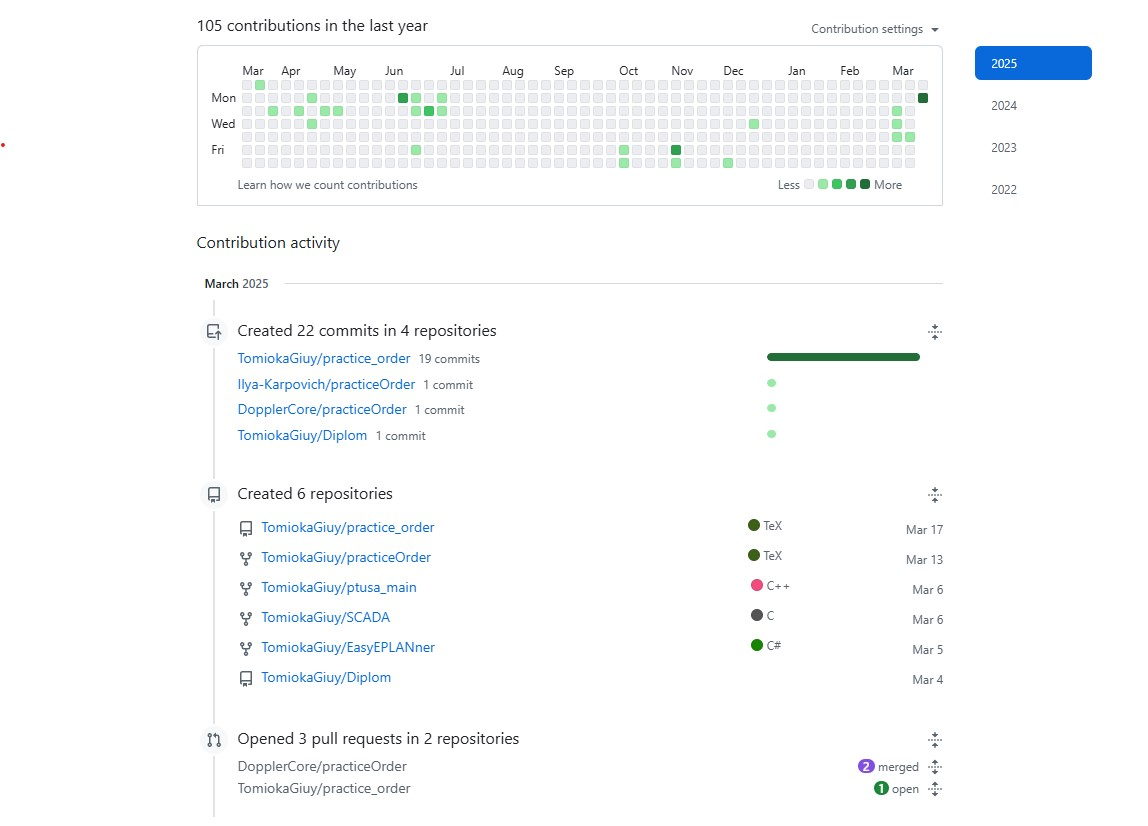
\includegraphics[width=0.8\textwidth]{img/activity.jpg}
  \caption{-- Активность GitHub}
  \label{fig:example}
\end{figure}


\par }